\section{Graphics Programming}


\subsection{Rendering in the browser}
\begin{table}[]
    \begin{tabular}{lllll}
        \hline
        technology   & use-case                    & programming style &                                                                                                                                                                 & libraries           \\ \hline
        canvas/2d    &                             &                   & single-buffering to bitmap. paintbrush-statemachine.                                                                                                            &                     \\
        canvas/webgl & 3d, interactive, many items & procedural        & double-buffering to bitmap                                                                                                                                      & threejs, processing \\
        svg + css    & simple 2d graphics          & declarative       & no bitmap, but \textbackslash{}inlinecode\{\textless{}svg\textgreater{}\}. has concept of layers, browser-native event-handling. Cannot easily export to image. & d3, raphael         \\ \hline
    \end{tabular}
\end{table}


\subsection{SVG}

SVG consists of 
\begin{itemize}
    \item Objects
    \item Groups. Groups have ...
        \begin{itemize}
            \item a transform
            \item a style
            \item Notably, they don't have a x, y, width or height attribute! If you need those, use SVG's instead
        \end{itemize}
    \item SVG's. 
        \begin{itemize}
            \item x, y width, height
        \end{itemize}
\end{itemize}

Objects have a nice, simple hierarchy.
\begin{itemize}
    \item Objects: each object is a ...
        \begin{itemize}
            \item Path: the most basic object: a Bezier-curve. Each of the following subtypes can be downgraded to a path again in inkscape.
                \begin{itemize}
                    \item rect, star, ellipse, text
                \end{itemize}
        \end{itemize}
    \item Each object has a ... 
        \begin{itemize}
            \item fill, stroke, opacity
        \end{itemize}
\end{itemize}

A bunch of software helps with SVG's:
\begin{itemize}
    \item Inkscape: ideal for creating SVG logos
    \item d3: Data-driven, animated SVG's
    \item Raphael: animated SVG's; imperative, \emph{not} data-driven
\end{itemize}


\subsection{D3}

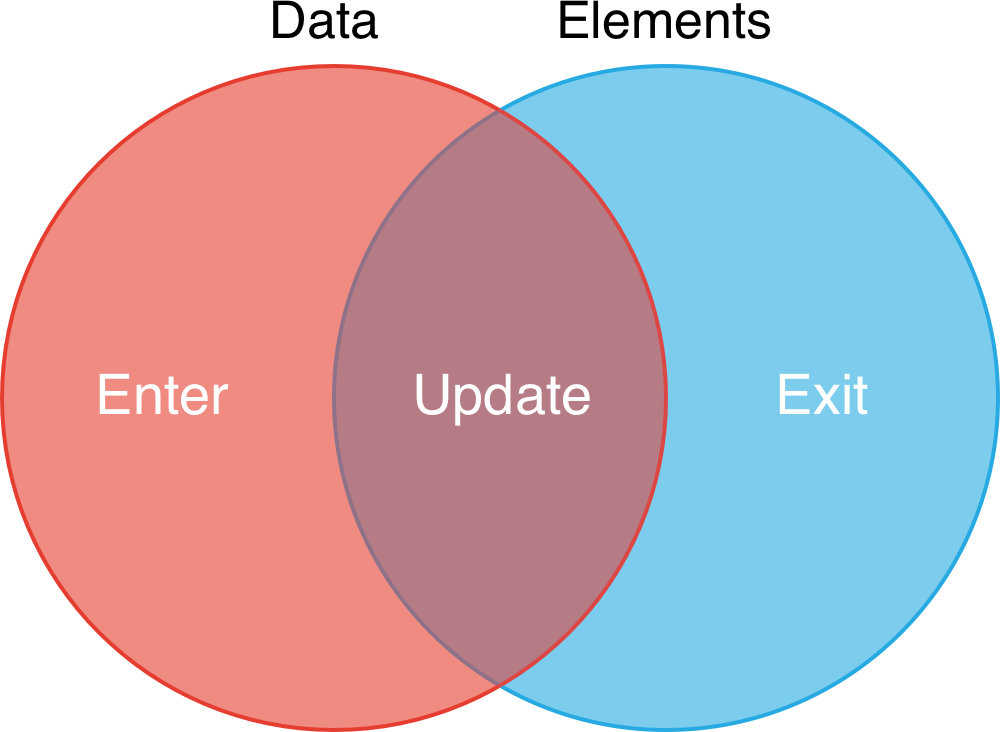
\includegraphics[width=0.3\textwidth]{d3_enter_update_exit.png}

\begin{lstlisting}
    <html>
    <head>
        <script src="https://d3js.org/d3.v6.js"></script>
    </head>
    <body>
        <h1>Demonstrating the selection, enter & exit flow for animations</h1>

        <ul id="list">
            <li>one</li>
            <li>two</li>
        </ul>

        <p>
            To explore this behavior, call `displayData` a few times from the web-console.
        </p>
    </body>
    <script>
        function displayData(data) {
            // step 1: create element- & data-selections (= the blue and the red cirlce)
            const elsNdata = d3.select('#list')  // selection of parent element
                .selectAll('li')  // select all child elements: [li, li]
                .data(data);

            // step 2: handle li's that already have (possibly old) data on them
            elsNdata
                .text(d => d);
            // usually, there are initially no pre-defined li's, such that this step is not required.
            // this is good for performance: not handling old items saves on dom-operations.
    
            // step 3: handle new data points coming in
            elsNdata.enter()  // all data points that have not yet got an associated li
                    .append('li')
                    .text(d => d);
            
            // step 4: handle old data points going out
            elsNdata.exit() // all li's that no longer have data on them
                .remove();
        }

        displayData([1, 2, 3])
    </script>
</html>
\end{lstlisting}


\begin{lstlisting}
    import { select, BaseType, EnterElement, Selection } from 'd3';


    // https://www.youtube.com/watch?v=IyIAR65G-GQ&t=1841s 
    
    interface DataPoint {
        id: number;
        value: number;
    }
    
    class Queue<T> {
        private data: T[];
        
        constructor(length: number) {
            this.data = Array(length);
        }
    
        push(val: T): T {
            this.data.push(val);
            return this.data.shift();
        }
    
        getData(): T[] {
            return this.data;
        }
    }
    
    const dataQueue = new Queue<DataPoint>(10);
    
    let id = 0;
    function addRandomData(queue: Queue<DataPoint>) {
        id += 1;
        queue.push({
            id: id,
            value: Math.random() * 10
        });
    }
    
    for (let i = 0; i < 10; i++) {
        addRandomData(dataQueue);
    }
    
    const baseElement: Selection<SVGElement, unknown, HTMLElement, any> = select('#svg')
        .attr('width', 300)
        .attr('height', 300)
        .append('g');
        
    function update(data: DataPoint[]) {
        
        // we need to re-select on every update cycle
        const circles: Selection<BaseType, unknown, SVGElement, unknown> = baseElement.selectAll('circle');
        const circlesWithData: Selection<BaseType, DataPoint, SVGElement, unknown> = circles
            .data(data, 
                // keyFunction: returns an id for each datum, so that elements know what data they are associated with
                (d: DataPoint, i: number, g: (SVGElement | BaseType)[]) => d.id
            );
        
        const entering: Selection<EnterElement, DataPoint, SVGElement, unknown> = circlesWithData.enter();
        const updating: Selection<BaseType, DataPoint, SVGElement, unknown> = circlesWithData;
        const enteringAndUpdating = updating.merge(entering);
        const leaving: Selection<BaseType, unknown, SVGElement, unknown> = circlesWithData.exit();
        console.log(`in: ${entering.size()} - update: ${updating.size()} - out: ${leaving.size()}`)
        
        const entered: Selection<SVGCircleElement, DataPoint, SVGElement, unknown> = entering
            .append('circle')
            .attr('r', 10)
            .attr('cx', (d, i) => i * 20)
            .attr('cy', (d) => 250 - d.value * 10)
            .attr('fill', 'green');
    
        const updated: Selection<BaseType, DataPoint, SVGElement, unknown> = updating
            .attr('cx', (d, i) => i * 10);
        
        const removed: Selection<BaseType, unknown, SVGElement, unknown> = leaving.remove();
    }
    
    const button = document.getElementById('button') as HTMLButtonElement;
    button.addEventListener('click', () => {
        addRandomData(dataQueue);
        const newData = dataQueue.getData();
        update(newData);
    }); 
\end{lstlisting}

\subsubsection{Updates}
A \inlinecode{Selection}s groups (update, enter and exit) stay the same, even if the data has already been modified.
To get the newer entries in the `update` group, you need to make a new \inlinecode{Selection} using \inlinecode{.selectAll('someTag')}.

\subsubsection{Call}
Call is a synonym to `tap`: it allows you to have a side-effect on a selection without breaking the method chain.

\begin{lstlisting}
selectAll('circle')
    .call(doWithSelection, 'red');

function doWithSelection(selection, color) {
    selection.attr('fill', color);
}
\end{lstlisting}

\subsubsection{Join}


\subsubsection{Range \& scale}


\subsection{Force}
One of the hardest parts of d3 is the usage of force in combination with drag.
\begin{lstlisting}
    import { BaseType, forceCenter, forceLink, forceManyBody, select, Selection } from "d3";
import { forceSimulation, SimulationLinkDatum, SimulationNodeDatum } from "d3-force";
import { drag } from 'd3-drag';

/**
Each node must be an object. The following properties are assigned by the simulation:

index: the node's zero-based index into nodes
x - the node's current x-position
y - the node's current y-position
vx - the node's current x-velocity
vy - the node's current y-velocity

The position (x, y) and velocity (vx, vy) may be subsequently modified by forces and by the simulation.
If either vx or vy is NaN, the velocity is initialized to (0, 0). If either x or y is NaN,
the position is initialized in a phyllotaxis arrangement, so chosen to ensure a deterministic, uniform distribution.

Each link is an object with the following properties:

source - the link's source node; see simulation.nodes
target - the link's target node; see simulation.nodes
 */

interface Institute extends SimulationNodeDatum {
    id: string;
}

const institutes: Institute[] = [{
    id: 'finance'
}, {
    id: 'spaceflight'
}, {
    id: 'research'
}];

const links: SimulationLinkDatum<Institute>[] = [{
    source: institutes.find(i => i.id === 'spaceflight'),
    target: institutes.find(i => i.id === 'finance')
}, {
    source: institutes.find(i => i.id === 'spaceflight'),
    target: institutes.find(i => i.id === 'research')
}];




const simulation = forceSimulation(institutes)
    .force("charge", forceManyBody().strength(-30))
    .force("link", forceLink(links))
    .force("center", forceCenter().x(150).y(150))
    .on('tick', simulationTick);

const dragCallback = drag()
    .on('start', (evt: DragEvent, d: Institute) => {
        simulation.alphaTarget(0.3).restart(); 
    })
    .on('drag', (evt, d: Institute) => {
        d.fx = evt.x;
        d.fy = evt.y;
    })
    .on('end', (evt: DragEvent, d: Institute) => {
        simulation.alphaTarget(0);
        d.fx = null;
        d.fy = null;
    });


const rootElement = select('#svg')
    .attr('width', 500)
    .attr('height', 300)
    .append('g');

rootElement.selectAll('circle')
    .data(institutes)
    .enter()
        .append('circle')
        .attr('r', 10)
        .call(dragCallback);

rootElement.selectAll('line')
    .data(links)
    .enter()
        .append('line')
        .attr('stroke', 'black')
        .attr('stroke-width', 2);

function simulationTick() {
    rootElement.selectAll('circle')
        .attr('cx', d => (d as Institute).x)
        .attr('cy', d => (d as Institute).y);

    rootElement.selectAll('line')
        .attr('x1', d => ((d as SimulationLinkDatum<Institute>).source as Institute).x)
        .attr('y1', d => ((d as SimulationLinkDatum<Institute>).source as Institute).y)
        .attr('x2', d => ((d as SimulationLinkDatum<Institute>).target as Institute).x)
        .attr('y2', d => ((d as SimulationLinkDatum<Institute>).target as Institute).y);
}
\end{lstlisting}

\subsection{Layout}
Layout is a way how d3 arranges data for you - commonly in a tree, or a circle-diagram or comparable. First you wrap your data in a \inlinecode{hierarchy}, then you call a layout-function (like for example \inlinecode{cluster}) on it.
\begin{lstlisting}
    import { select, cluster, curveBundle, lineRadial, dsv, hierarchy } from 'd3';


    const width = 700;
    const height = 500;
    const circleRadius = 200;
    
    
    function findInTree(name, parentGroupName, tree) {
        const parentGroup = tree.children.find(e => e.name === parentGroupName);
        if (parentGroup) {
            const entry = parentGroup.children.find(e => e.name === name);
            return entry;
        }
    }
    
    function addToTree(name, parentGroupName, tree) {
        const parentGroup = tree.children.find(e => e.name === parentGroupName);
        parentGroup.children.push({
            name, parentGroupName,
            in: [],
            out: []
        });
    }
    
    function findInHierarchy(name, groupName, hierarchy) {
        const group = hierarchy.children.find(c => c.data.name === groupName);
        if (group) {
            const child = group.children.find(c => c.data.name === name);
            return child;
        }
    }
    
    function parseDataInTree(data) {
    
        // step 0: base data
        const base = {
            name: 'base',
            children: [{
                name: 'cluster',
                children: []
            }, {
                name: 'project',
                children: []
            }, {
                name: 'potential',
                children: []
            }, {
                name: 'institute',
                children: []
            }]
        };
    
        // step 1: hierarchy
        for (let row of data) {
            const institute = row['DLR Institut'];
            if (!findInTree(institute, 'institute', base)) {
                addToTree(institute, 'institute', base);
            }
            const potential = row['Potential'];
            if (!findInTree(potential, 'potential', base)) {
                addToTree(potential, 'potential', base);
            }
            const project = row['Projekt'];
            if (!findInTree(project, 'project', base)) {
                addToTree(project, 'project', base);
            }
            const cluster = row['HumTech Cluster (UNHCR)'];
            if (!findInTree(cluster, 'cluster', base)) {
                addToTree(cluster, 'cluster', base);
            }
    
        }
        const hierarchyData = hierarchy(base);
    
        // step 2: connections at leaf-level
        for (let row of data) {
            const institute = row['DLR Institut'];
            const potential = row['Potential'];
            const project = row['Projekt'];
            const cluster = row['HumTech Cluster (UNHCR)'];
    
            if (institute && potential) {
                const startNode = findInHierarchy(institute, 'institute', hierarchyData);
                const targetNode = findInHierarchy(potential, 'potential', hierarchyData);
                startNode.data.out.push(targetNode);
                targetNode.data.in.push(startNode);
            }
    
            if (institute && project) {
                const startNode = findInHierarchy(institute, 'institute', hierarchyData);
                const targetNode = findInHierarchy(project, 'project', hierarchyData);
                startNode.data.out.push(targetNode);
                targetNode.data.in.push(startNode);
            }
    
            if (project && cluster) {
                const startNode = findInHierarchy(project, 'project', hierarchyData);
                const targetNode = findInHierarchy(cluster, 'cluster', hierarchyData);
                startNode.data.out.push(targetNode);
                targetNode.data.in.push(startNode);
            }
    
            if (potential && cluster) {
                const startNode = findInHierarchy(potential, 'potential', hierarchyData);
                const targetNode = findInHierarchy(cluster, 'cluster', hierarchyData);
                startNode.data.out.push(targetNode);
                targetNode.data.in.push(startNode);
            }
        }
    
        return hierarchyData;
    }
    
    function getBubbleColor(d) {
        if (d.depth === 2) {
            switch (d.parent.data.name) {
                case 'cluster':
                    return 'yellow';
                case 'project':
                    return 'blue';
                case 'institute':
                    return 'green';
                case 'potential':
                    return 'red';
            }
        } else if (d.depth === 1) {
            return 'black';
        } else {
            return 'black';
        }
    }
    
    function getPathsFromTree(treeData) {
        const paths = [];
    
        for (let source of treeData.leaves()) {
            for (let target of source.data.out) {
                const path = source.path(target);
                paths.push(path);
            }
        }
    
        return paths;
    }
    
    function getConnectedPaths(node) {
        const paths = [];
        for (let input of node.data.in) {
            const path = input.path(node);
            paths.push(path);
        }
        for (let output of node.data.out) {
            const path = output.path(node);
            paths.push(path);
        }
        return paths;
    }
    
    function getConnectedNodes(node) {
        const nodes = [];
        for (let input of node.data.in) {
            nodes.push(input);
        }
        for (let output of node.data.out) {
            nodes.push(output);
        }
        return nodes;
    }
    
    
    async function main() {
        function highlightConnections(connectedPaths) {
            const highlightedConnections = baseElement
                .selectAll('.highlightedConnection')
                .data(connectedPaths);
            highlightedConnections
                .enter()
                    .append('path')
                    .attr('class', 'highlightedConnection')
                    .attr('d', connectionPathFunction)
                    .attr('stroke', 'black')
                    .attr('fill', 'none')
            highlightedConnections
                .exit()
                    .remove();
        }
    
        function highlightNodes(nodes) {
            const highlightedNodes = baseElement
                .selectAll('.highlightedNode')
                .data(nodes);
            highlightedNodes
                .enter()
                    .append('circle')
                    .attr('class', 'highlightedNode')
                    .attr('r', 15)
                    .attr('transform', d => `rotate(${d.x - 90}) translate(${d.y}, 0)`)
                    .attr('fill', 'black');
            highlightedNodes
                .exit()
                    .remove();
        }
    
        function onMouseOver(evt, d) {
            const connectedPaths = getConnectedPaths(d);
            const connectedNodes = getConnectedNodes(d);
            highlightConnections(connectedPaths);
            highlightNodes(connectedNodes);
        }
        
        function onMouseOut(evt, d) {
            highlightConnections([]);
            highlightNodes([]);
        }
    
        const data = await dsv('|', './data2.csv');
    
        const treeData = parseDataInTree(data);
        const pathData = getPathsFromTree(treeData);
    
        const baseElement = select('#graphic')
            .attr('width', width)
            .attr('height', height)
            .append('g')
            .attr('transform', `translate(${width / 2} ${height / 2})`);
    
        const circlePositioningFunction = cluster()
            .size([360, circleRadius]);
        const treeDataWithPositions = circlePositioningFunction(treeData);
        const leafDataWithPositions = treeDataWithPositions.leaves();
    
        const connectionPathFunction = lineRadial()
            .curve(curveBundle.beta(0.7))
            .radius(d => d.y)
            .angle(d => d.x / 180 * Math.PI);
    
        const connections = baseElement
            .selectAll('.connection')
            .data(pathData)
            .enter()
            .append('path')
            .attr('class', 'connection')
            .attr('d', connectionPathFunction)
            .attr('stroke', 'gray')
            .attr('fill', 'none');
    
        const circles = baseElement
            .selectAll('.bubble')
            .data(leafDataWithPositions)
            .enter()
            .append('circle')
            .attr('class', 'bubble')
            .attr('r', 10)
            .attr('fill', d => getBubbleColor(d))
            .attr('stroke', 'black')
            .attr('transform', d => `rotate(${d.x - 90}) translate(${d.y}, 0)`)
            .on('mouseover', onMouseOver)
            .on('mouseout', onMouseOut);
    
    }
    
    main();
\end{lstlisting}


\subsection{WASM}

\begin{itemize}
    \item Module: compiled WASM. Can be passed around. Stateless.
    \item Instance: a module + it's state
    \item State: 
        \begin{itemize}
            \item Memory: resizable ArrayBuffer
            \item Table: array of references to functions
        \end{itemize}
\end{itemize}

\begin{itemize}
    \item Calls from js to wasm are synchronous.
\end{itemize}

\begin{itemize}
    \item LLVM: compiles C to intermediate (via the Clang-Frontend) and intermediate to WASM (via the WASM-Backend)
    \item Emscripten: includes LLVM. But also creates custom JS to be used by WASM to emulate \inlinecode{stdio} et.al.
    \begin{itemize} 
        \item Really, this includes all of \inlinecode{libc}, including \inlinecode{ malloc()} and \inlinecode{free()}.
    \end{itemize}
\end{itemize}


\begin{lstlisting}[language=c]
int add (int a, int b) {
    return a*a + b;
}

float int_arraySum (int* array, int length) {
    float total = 0; 
    for (int i = 0; i < length; i++) {
        total += array[i];
    }
    return total;
}

void int_arrayAddition (int* arr1, int* arr2, int* arrSum, int arrLength) {
    for (int i = 0; i < arrLength; i++) {
        arrSum[i] = arr1[i] + arr2[i];
    }
}

float float_arraySum (float* array, int length) {
    float total = 0; 
    for (int i = 0; i < length; i++) {
        total += array[i];
    }
    return total;
}

void float_arrayAddition (float* arr1, float* arr2, float* arrSum, int arrLength) {
    for (int i = 0; i < arrLength; i++) {
        arrSum[i] = arr1[i] + arr2[i];
    }
}
\end{lstlisting}

\begin{lstlisting}[language=bash]
    clang --target=wasm32 -O3 -flto -nostdlib -Wl,--no-entry -Wl,--export-all -Wl,--lto-O3 -o prog.wasm prog.c
\end{lstlisting}

\begin{lstlisting}[language=java]
    const memory = new WebAssembly.Memory({
        initial: 100, // in pages (64KiB / Page)
        maximum: 1000
    });
    
    WebAssembly.instantiateStreaming(fetch('prog.wasm'), {
        js: {
            mem: memory
        }
    }).then((response) => {
        console.log(response);
    
    
        // simple function
        const result1 = response.instance.exports.add(4, 1);
        console.log(`4**2 + 1`, result1);
    
    
    
    
        // pointer to top of memory array
        let offsetBytes = 0;
        const memBuf = response.instance.exports.memory.buffer;
    
    
    
        // wasm accesses js data
        const data1 = [1, 2, 3, 4.4, 5];
        const arr1 = new Float32Array(memBuf, offsetBytes, data1.length);
        arr1.set(data1);
        offsetBytes += arr1.length * arr1.BYTES_PER_ELEMENT;
        
        const result2 = response.instance.exports.float_arraySum(arr1.byteOffset, arr1.length);
        console.log(`sum of (${arr1})`, result2);
    
    
    
    
        // js accesses wasm data
        const l = 3;
    
        const data2 = [1, 2, 3.1];
        const arr2 = new Float32Array(memBuf, offsetBytes, l);
        arr2.set(data2);
        offsetBytes += arr2.length * arr2.BYTES_PER_ELEMENT;
    
        const data3 = [4, 5.1, 6];
        const arr3 = new Float32Array(memBuf, offsetBytes, l);
        arr3.set(data3);
        offsetBytes += arr3.length * arr3.BYTES_PER_ELEMENT;
    
        const arr4 = new Float32Array(memBuf, offsetBytes, l);
        offsetBytes += arr4.length * arr4.BYTES_PER_ELEMENT;
    
        response.instance.exports.float_arrayAddition(arr2.byteOffset, arr3.byteOffset, arr4.byteOffset, l);
        console.log(`addition of ${arr2} and ${arr3} = `, arr4)
        
    });
\end{lstlisting}


\subsection{WebGl}

\begin{lstlisting}
    import { flattenMatrix } from './engine.shapes';

    /**
     * WEBGL
     *
     * A rasterization engine that allows to draw points, line segments, or triangles.
     *
     * Vertex shaders take whatever coordinates you use and return a 3-d array with elements between -1 and 1.
     * Basically, this is a 3d-array, but WebGl does not use the z-axis for real perspective, but only to differentiate
     * what pixel lies in front of another.
     * This is not like looking in a 3d-box, but rather like looking on multiple stacked sheets on a projector.
     * Actually, this is a lie. WebGl uses 4 coordinates: x, y, z and w. The above only holds if you keep w at 1.
     * After applying the vertex shader, WebGl divides all coordinates by w, yielding (x/w, y/w, z/w, 1).
     * This can be used to calculate projections - google for 'homogeneous coordinates' to find out more.
     * Compare this [site](https://www.tomdalling.com/blog/modern-opengl/explaining-homogenous-coordinates-and-projective-geometry/)
     * and the shader `basic3d.vert.glsl`.
     *
     * WebGL knows two data structures:
     *  - buffers (generic byte arrays): usually positions, normals, texture-coordinates, vertex-colors etc.
     *    buffers are accessed in shaders as 'attributes'.
     *    note that buffers contain one entry for each vertex.
     *  - textures (bitmap images).
     *
     * Shaders use these data structures in two different ways.
     *  - Attributes are values, one per vertex.
     *    For the shader, attributes are read-only.
     *    Attributes default to [0, 0, 0, 1]
     *  - Uniforms are values, one per shader.
     *    For the shader, uniforms are read-only.
     *
     * Apart from this, shaders know about two more types of data:
     *  - Varyings are values that are passed from vertex-shader to fragment-shader.
     *    They are read-only only for the fragment-shader.
     *  - Const: a compile-time constant.
     *
     * A program is just a list of compiled and linked vertex- and fragment-shaders.
     *
     *
     * Drawing: there's drawArrays and drawElements.
     *  - drawArrays is the robust all-rounder.
     *  - drawElements can be more performant if you share vertices between objects.
     *
     *
     * Rendering data is fast, but uploading it into GPU memory is slow.
     * Optimizing WebGl performance mostly means: Avoiding having GPU and CPU wait for each other.
     * The more the GPU can do in bulk, the better. The more often you have to upload data from CPU to GPU, the worse.
     *  - So avoid switching programs, buffers and uniforms if you can.
     *    (You won't be able to avoid switching buffers, because every object is likely different. But sort your objects by their shaders, and you'll save a lot of time.)
     *  - Try to do translations, rotations and shears inside the vertex-shader instead of altering the object's buffer.
     *  - If appropriate, create ueber-shaders and ueber-buffers, that contain information for more than just one object.
     *
     * There is another thing that affects performance:
     * WebGL will only run fragment-shaders when the object's pixels aren't already obscured by a larger object in front of it.
     * That means it makes sense to first draw large objects that are close to the camera - all objects behind them won't need their fragment-shader executed.
     *
     * All `create*` functions unbind variables after setting their values. This is to avoid unwanted side-effects.
     */
    
    
    
    const shaderInputTextureBindPoint = 0;
    const textureConstructionBindPoint = 7;
    
    
    
    
    /**
     * Compile shader.
     */
    export const compileShader = (gl: WebGLRenderingContext, typeBit: number, shaderSource: string): WebGLShader => {
        const shader = gl.createShader(typeBit);
        if (!shader) {
            throw new Error('No shader was created');
        }
        gl.shaderSource(shader, shaderSource);
        gl.compileShader(shader);
        if (!gl.getShaderParameter(shader, gl.COMPILE_STATUS)) {
            gl.deleteShader(shader);
            throw new Error(`An error occurred compiling the shader: ${gl.getShaderInfoLog(shader)}.    \n\n Shader code: ${shaderSource}`);
        }
        return shader;
    };
    
    
    /**
     * Note that every program *must* have one and only one vertex-shader
     * and one and only one fragment shader.
     * That means you cannot add multiple fragment-shaders in one program. Instead, either load them in consecutively as part of different programs,
     * or generate an ueber-shader that contains both codes.
     */
    export const createShaderProgram = (gl: WebGLRenderingContext, vertexShaderSource: string, fragmentShaderSource: string): WebGLProgram => {
    
        const program = gl.createProgram();
        if (!program) {
            throw new Error('No program was created');
        }
    
        const vertexShader = compileShader(gl, gl.VERTEX_SHADER, vertexShaderSource);
        const fragmentShader = compileShader(gl, gl.FRAGMENT_SHADER, fragmentShaderSource);
        gl.attachShader(program, vertexShader);
        gl.attachShader(program, fragmentShader);
    
        gl.linkProgram(program);
    
        gl.detachShader(program, vertexShader);
        gl.detachShader(program, fragmentShader);
        gl.deleteShader(vertexShader);
        gl.deleteShader(fragmentShader);
    
        if (!gl.getProgramParameter(program, gl.LINK_STATUS)) {
            gl.deleteProgram(program);
            throw new Error('Unable to initialize the shader program: ' + gl.getProgramInfoLog(program));
        }
    
        return program;
    };
    
    
    export const setup3dScene = (gl: WebGLRenderingContext): void => {
        gl.viewport(0, 0, gl.canvas.width, gl.canvas.height);  // making sure that shader-coordinate-system goes from 0 to 1.
    
        gl.enable(gl.DEPTH_TEST);
        gl.depthFunc(gl.LEQUAL);
        gl.cullFace(gl.BACK);
    
        clearBackground(gl, [0, 0, 0, 1]);
    };
    
    
    export const bindProgram = (gl: WebGLRenderingContext, program: WebGLProgram): void => {
        gl.useProgram(program);
    };
    
    
    export const clearBackground = (gl: WebGLRenderingContext, color: number[]): void => {
        gl.clearColor(color[0], color[1], color[2], color[3]);
        gl.clearDepth(1.0);
        gl.clear(gl.COLOR_BUFFER_BIT | gl.DEPTH_BUFFER_BIT);
    };
    
    
     /**
      * A generic buffer, together with it's metadata.
      */
    export interface BufferObject {
        buffer: WebGLBuffer;
        vectorSize: number;
        vectorCount: number;
        type: number;
        normalize: boolean;
        stride: number;
        offset: number;
        drawingMode: number; // gl.TRIANGLES, gl.POINTS, or gl.LINES
    }
    
    
    /**
     * Create buffer. Creation is slow! Do *before* render loop.
     */
    export const createFloatBuffer = (gl: WebGLRenderingContext, data: number[][], drawingMode: number = gl.TRIANGLES): BufferObject => {
    
        const dataFlattened = new Float32Array(flattenMatrix(data));
    
        const buffer = gl.createBuffer();
        if (!buffer) {
            throw new Error('No buffer was created');
        }
        gl.bindBuffer(gl.ARRAY_BUFFER, buffer);
        gl.bufferData(gl.ARRAY_BUFFER, dataFlattened, gl.STATIC_DRAW);
        // STATIC_DRAW: tells WebGl that we are not likely to change this data much.
        gl.bindBuffer(gl.ARRAY_BUFFER, null);  // unbinding
    
        const bufferObject: BufferObject = {
            buffer: buffer,
            vectorSize: data[0].length,
            vectorCount: data.length,
            type: gl.FLOAT,   // the data is 32bit floats
            normalize: false, // don't normalize the data
            stride: 0,        // 0 = move forward size * sizeof(type) each iteration to get the next position. Only change this in very-high-performance jobs.
            offset: 0,        // start at the beginning of the buffer. Only change this in very-high-performance jobs.
            drawingMode: drawingMode
        };
    
        return bufferObject;
    };
    
    
    export const drawArray = (gl: WebGLRenderingContext, bo: BufferObject): void => {
        gl.drawArrays(bo.drawingMode, bo.offset, bo.vectorCount);
    };
    
    
    
    export const updateBufferData = (gl: WebGLRenderingContext, bo: BufferObject, newData: number[][]): BufferObject => {
    
        const dataFlattened = new Float32Array(flattenMatrix(newData));
    
        gl.bindBuffer(gl.ARRAY_BUFFER, bo.buffer);
        gl.bufferData(gl.ARRAY_BUFFER, dataFlattened, gl.STATIC_DRAW);
        gl.bindBuffer(gl.ARRAY_BUFFER, null);  // unbinding
    
        const newBufferObject: BufferObject = {
            buffer: bo.buffer,
            vectorSize: newData[0].length,
            vectorCount: newData.length,
            type: gl.FLOAT,   // the data is 32bit floats
            normalize: false, // don't normalize the data
            stride: 0,        // 0 = move forward size * sizeof(type) each iteration to get the next position. Only change this in very-high-performance jobs.
            offset: 0,        // start at the beginning of the buffer. Only change this in very-high-performance jobs.
            drawingMode: bo.drawingMode,
        };
    
        return newBufferObject;
    };
    
    
    
    
    /**
     * Fetch attribute's location (attribute declared in some shader). Slow! Do *before* render loop.
     */
    export const getAttributeLocation = (gl: WebGLRenderingContext, program: WebGLProgram, attributeName: string): number => {
        const loc = gl.getAttribLocation(program, attributeName);
        if (loc === -1) {
            throw new Error(`Couldn't find attribute ${attributeName} in program.`);
        }
        return loc;
    };
    
    
    
    /**
     * Attributes vary from vertex to vertex - that means that there are *many* of them.
     * So it makes sense for WebGl to store attribute values in a dedicated data structure - the buffer.
     */
    export const bindBufferToAttribute = (gl: WebGLRenderingContext, attributeLocation: number, bufferObject: BufferObject): void => {
        // Enable editing
        gl.enableVertexAttribArray(attributeLocation);
        // Bind buffer to ARRAY_BUFFER
        gl.bindBuffer(gl.ARRAY_BUFFER, bufferObject.buffer);
        // Bind the buffer currently at ARRAY_BUFFER to a vertex-buffer-location.
        gl.vertexAttribPointer(
            attributeLocation,
            bufferObject.vectorSize, bufferObject.type, bufferObject.normalize, bufferObject.stride, bufferObject.offset);
        // gl.disableVertexAttribArray(attributeLocation); <-- must not do this!
    };
    
    
    
    
    export interface IndexBufferObject {
        buffer: WebGLBuffer;
        count: number;
        type: number; // must be gl.UNSIGNED_SHORT
        offset: number;
        drawingMode: number; // gl.TRIANGLES, gl.POINTS, or gl.LINES
    }
    
    export const createIndexBuffer = (gl: WebGLRenderingContext, indices: number[][], drawingMode: number = gl.TRIANGLES): IndexBufferObject => {
    
        const indicesFlattened = new Uint16Array(flattenMatrix(indices));
    
        const buffer = gl.createBuffer();
        if (!buffer) {
            throw new Error('No buffer was created');
        }
        gl.bindBuffer(gl.ELEMENT_ARRAY_BUFFER, buffer);
        gl.bufferData(gl.ELEMENT_ARRAY_BUFFER, indicesFlattened, gl.STATIC_DRAW);
        gl.bindBuffer(gl.ELEMENT_ARRAY_BUFFER, null);
    
        const bufferObject: IndexBufferObject = {
            buffer: buffer,
            count: indicesFlattened.length,
            type: gl.UNSIGNED_SHORT,
            offset: 0,
            drawingMode: drawingMode
        };
    
        return bufferObject;
    };
    
    export const drawElements = (gl: WebGLRenderingContext, ibo: IndexBufferObject): void => {
        gl.bindBuffer(gl.ELEMENT_ARRAY_BUFFER, ibo.buffer);  // @TODO: optimize this to somewhere else?
        gl.drawElements(ibo.drawingMode, ibo.count, ibo.type, ibo.offset);
    };
    
    
    export const draw = (gl: WebGLRenderingContext, b: BufferObject | IndexBufferObject): void => {
        if (b.type  === gl.UNSIGNED_SHORT) {
            drawElements(gl, b as IndexBufferObject);
        } else {
            drawArray(gl, b as BufferObject);
        }
    };
    
    
    
    
    
    export interface TextureObject {
        texture: WebGLTexture;
        width: number;
        height: number;
        level: number;
        internalformat: number;
        format: number;
        type: number;
    }
    
    /**
     * A shader's attributes get their buffer-values from the VERTEX_ARRAY, but they are constructed in the ARRAY_BUFFER.
     * Textures analogously are served from the TEXTURE_UNITS, while for construction they are bound to ACTIVE_TEXTURE.
     *
     * There is a big difference, however. Contrary to buffers which receive their initial value while still outside the ARRAY_BUFFER,
     * a texture does already have to be bound into the TEXTURE_UNITS when it's being created.
     * Since it'll always be bound into the slot that ACTIVE_TEXTURE points to, you can inadvertently overwrite another texture that is
     * currently in this place. To avoid this, we provide a dedicated `textureConstructionBindPoint`.
     *
     * Buffers are easier in this, since with vertexAttribPointer we are guaranteed to get a slot in the VERTEX_ARRAY that is not
     * already occupied by another buffer.
     */
    export const createTexture = (gl: WebGLRenderingContext, image: HTMLImageElement | HTMLCanvasElement): TextureObject => {
    
        const texture = gl.createTexture();  // analog to createBuffer
        if (!texture) {
            throw new Error('No texture was created');
        }
        gl.activeTexture(gl.TEXTURE0 + textureConstructionBindPoint); // so that we don't overwrite another texture in the next line.
        gl.bindTexture(gl.TEXTURE_2D, texture);  // analog to bindBuffer. Binds texture to currently active texture-bindpoint (aka. texture unit).
        gl.texImage2D(gl.TEXTURE_2D, 0, gl.RGBA, gl.RGBA, gl.UNSIGNED_BYTE, image);  // analog to bufferData
        gl.generateMipmap(gl.TEXTURE_2D); // mipmaps are mini-versions of the texture.
        gl.bindTexture(gl.TEXTURE_2D, null);  // unbinding
    
        let w, h: number;
        if (image instanceof HTMLImageElement) {
            w = image.naturalWidth;
            h = image.naturalHeight;
        } else {
            w = image.width;
            h = image.height;
        }
    
        const textureObj: TextureObject = {
            texture: texture,
            level: 0,
            internalformat: gl.RGBA,
            format: gl.RGBA,
            type: gl.UNSIGNED_BYTE,
            width: w,
            height: h
        };
    
        return textureObj;
    };
    
    
    
    export const createEmptyTexture = (gl: WebGLRenderingContext, width: number, height: number): TextureObject => {
        if (width <= 0 || height <= 0) {
            throw new Error('Width and height must be positive.');
        }
        const texture = gl.createTexture();
        if (!texture) {
            throw new Error('No texture was created');
        }
        gl.activeTexture(gl.TEXTURE0 + textureConstructionBindPoint); // so that we don't overwrite another texture in the next line.
        gl.bindTexture(gl.TEXTURE_2D, texture);
        gl.texImage2D(gl.TEXTURE_2D, 0, gl.RGBA, width, height, 0, gl.RGBA, gl.UNSIGNED_BYTE, null);
        gl.texParameteri(gl.TEXTURE_2D, gl.TEXTURE_WRAP_S, gl.CLAMP_TO_EDGE);
        gl.texParameteri(gl.TEXTURE_2D, gl.TEXTURE_WRAP_T, gl.CLAMP_TO_EDGE);
        gl.texParameteri(gl.TEXTURE_2D, gl.TEXTURE_MIN_FILTER, gl.NEAREST);
        gl.texParameteri(gl.TEXTURE_2D, gl.TEXTURE_MAG_FILTER, gl.NEAREST);
        gl.bindTexture(gl.TEXTURE_2D, null);
    
        const textureObj: TextureObject = {
            texture: texture,
            level: 0,
            internalformat: gl.RGBA,
            format: gl.RGBA,
            type: gl.UNSIGNED_BYTE,
            width: width,
            height: height
        };
    
        return textureObj;
    };
    
    
    /**
     * Even though we reference textures as uniforms in a fragment shader, assigning an actual texture-value to that uniform works differently than for normal uniforms.
     * Normal uniforms have a concrete value.
     * Texture uniforms, on the other hand, are just an integer-index that points to a special slot in the GPU memory (the bindPoint) where the actual texture value lies.
     */
    export const bindTextureToUniform = (gl: WebGLRenderingContext, texture: WebGLTexture, bindPoint: number, uniformLocation: WebGLUniformLocation): void =>  {
        if (bindPoint > gl.getParameter(gl.MAX_COMBINED_TEXTURE_IMAGE_UNITS)) {
            throw new Error(`There are only ${gl.getParameter(gl.MAX_COMBINED_TEXTURE_IMAGE_UNITS)} texture bind points, but you tried to bind to point nr. ${bindPoint}.`);
        }
        if (bindPoint === textureConstructionBindPoint) {
            console.error(`You are about to bind to the dedicated texture-construction bind point (nr. ${bindPoint}).
            If after this call another texture is built, your shader will now use that new texture instead of this one!
            Consider using another bind point.`);
        }
        gl.activeTexture(gl.TEXTURE0 + bindPoint);  // analog to enableVertexAttribArray
        gl.bindTexture(gl.TEXTURE_2D, texture);  // analog to bindBuffer. Binds texture to currently active texture-bindpoint (aka. texture unit).
        gl.uniform1i(uniformLocation, bindPoint); // analog to vertexAttribPointer
    };
    
    
    
    export const updateTexture = (gl: WebGLRenderingContext, to: TextureObject, newImage: HTMLImageElement | HTMLCanvasElement): TextureObject => {
    
        gl.activeTexture(gl.TEXTURE0 + textureConstructionBindPoint); // so that we don't overwrite another texture in the next line.
        gl.bindTexture(gl.TEXTURE_2D, to.texture);  // analog to bindBuffer. Binds texture to currently active texture-bindpoint (aka. texture unit).
        gl.texImage2D(gl.TEXTURE_2D, 0, gl.RGBA, gl.RGBA, gl.UNSIGNED_BYTE, newImage);  // analog to bufferData
        gl.generateMipmap(gl.TEXTURE_2D); // mipmaps are mini-versions of the texture.
        gl.bindTexture(gl.TEXTURE_2D, null);  // unbinding
    
        let w, h: number;
        if (newImage instanceof HTMLImageElement) {
            w = newImage.naturalWidth;
            h = newImage.naturalHeight;
        } else {
            w = newImage.width;
            h = newImage.height;
        }
        to.width = w;
        to.height = h;
    
        return to;
    };
    
    
    export interface FramebufferObject {
        framebuffer: WebGLFramebuffer;
        texture: TextureObject;
        width: number;
        height: number;
    }
    
    
    export const createFramebuffer = (gl: WebGLRenderingContext): WebGLFramebuffer => {
        const fb = gl.createFramebuffer();  // analog to createBuffer
        if (!fb) {
            throw new Error(`Error creating framebuffer`);
        }
        return fb;
    };
    
    
    /**
     * The operations `clear`, `drawArrays` and `drawElements` only affect the currently bound framebuffer.
     */
    export const bindFramebuffer = (gl: WebGLRenderingContext, fbo: FramebufferObject) => {
        gl.bindFramebuffer(gl.FRAMEBUFFER, fbo.framebuffer);
        gl.viewport(0, 0, fbo.width, fbo.height);
        // Note that binding the framebuffer does *not* mean binding its texture. In fact, if there is a bound texture, it must be the *input* to a shader, not the output.
        // Therefore, a framebuffer's texture must not be bound when the framebuffer is.
    };
    
    
    export const bindOutputCanvasToFramebuffer = (gl: WebGLRenderingContext) => {
        gl.bindFramebuffer(gl.FRAMEBUFFER, null);
        gl.viewport(0, 0, gl.canvas.width, gl.canvas.height);
    };
    
    
    /**
     * A framebuffer can have a texture - that is the bitmap that the shader-*out*put is drawn on.
     * Shaders may also have one or more *in*put texture(s), which must be provided to the shader as a uniform sampler2D.
     * Only the shader needs to know about any potential input texture, the framebuffer will always only know about it's output texture.
     */
    export const bindTextureToFramebuffer = (gl: WebGLRenderingContext, texture: TextureObject, fb: WebGLFramebuffer): FramebufferObject => {
        gl.bindFramebuffer(gl.FRAMEBUFFER, fb);
        gl.framebufferTexture2D(gl.FRAMEBUFFER, gl.COLOR_ATTACHMENT0, gl.TEXTURE_2D, texture.texture, 0); // analog to bufferData
    
        if (gl.checkFramebufferStatus(gl.FRAMEBUFFER) !== gl.FRAMEBUFFER_COMPLETE) {
            throw new Error(`Error creating framebuffer: framebuffer-status: ${gl.checkFramebufferStatus(gl.FRAMEBUFFER)} ; error-code: ${gl.getError()}`);
        }
    
        gl.bindFramebuffer(gl.FRAMEBUFFER, null);
    
        const fbo: FramebufferObject = {
            framebuffer: fb,
            texture: texture,
            width: texture.width,
            height: texture.height
        };
    
        return fbo;
    };
    
    
    
    
    
    
    
    
    
    
    /**
     * Fetch uniform's location (uniform declared in some shader). Slow! Do *before* render loop.
     */
    export const getUniformLocation = (gl: WebGLRenderingContext, program: WebGLProgram, uniformName: string): WebGLUniformLocation => {
        const loc = gl.getUniformLocation(program, uniformName);
        if (loc === null) {
            throw new Error(`Couldn't find uniform ${uniformName} in program.`);
        }
        return loc;
    };
    
    
    
    
    export type UniformType = '1i' | '2i' | '3i' | '4i' | '1f' | '2f' | '3f' | '4f' | '1fv' | '2fv' | '3fv' | '4fv' | 'matrix2fv' | 'matrix3fv' | 'matrix4fv';
    
    /**
     * Contrary to attributes, uniforms don't need to be stored in a buffer.
     *
     * 'v' is not about the shader, but how you provide data from the js-side.
     * uniform1fv(loc, [3.19]) === uniform1f(loc, 3.19)
     *
     * |js                                      |          shader                  |
     * |----------------------------------------|----------------------------------|
     * |uniform1f(loc, 3.19)                    |  uniform float u_pi;             |
     * |uniform2f(loc, 3.19, 2.72)              |  uniform vec2 u_constants;       |
     * |uniform2fv(loc, [3.19, 2.72])           |  uniform vec2 u_constants;       |
     * |uniform1fv(loc, [1, 2, 3, 4, 5, 6])     |  uniform float u_kernel[6];      |
     * |uniform2fv(loc, [1, 2, 3, 4, 5, 6])     |  uniform vec2 u_observations[3]; |
     * |uniformMatrix3fv(loc, [[...], [...]])   |  uniform mat3 u_matrix;          |
     *
     */
    export const bindValueToUniform = (gl: WebGLRenderingContext, uniformLocation: WebGLUniformLocation, type: UniformType, values: number[]): void => {
        switch (type) {
            case '1i':
                gl.uniform1i(uniformLocation, values[0]);
                break;
    
            case '1f':
                gl.uniform1f(uniformLocation, values[0]);
                break;
            case '2f':
                gl.uniform2f(uniformLocation, values[0], values[1]);
                break;
            case '3f':
                gl.uniform3f(uniformLocation, values[0], values[1], values[2]);
                break;
            case '4f':
                gl.uniform4f(uniformLocation, values[0], values[1], values[2], values[3]);
                break;
    
            case '1fv':
                gl.uniform1fv(uniformLocation, values);
                break;
            case '2fv':
                gl.uniform2fv(uniformLocation, values);
                break;
            case '3fv':
                gl.uniform3fv(uniformLocation, values);
                break;
            case '4fv':
                gl.uniform4fv(uniformLocation, values);
                break;
    
            // In the following *matrix* calls, the 'transpose' parameter must always be false. 
            // Quoting the OpenGL ES 2.0 spec:
            // If the transpose parameter to any of the UniformMatrix* commands is
            // not FALSE, an INVALID_VALUE error is generated, and no uniform values are
            // changed.
            case 'matrix2fv':
                gl.uniformMatrix2fv(uniformLocation, false, values);
                break;
    
            case 'matrix3fv':
                gl.uniformMatrix3fv(uniformLocation, false, values);
                break;
    
            case 'matrix4fv':
                gl.uniformMatrix4fv(uniformLocation, false, values);
                break;
    
            default:
                throw Error(`Type ${type} not yet implemented.`);
        }
    };
    
    
    /**
     * (From https://hacks.mozilla.org/2013/04/the-concepts-of-webgl/ and https://stackoverflow.com/questions/56303648/webgl-rendering-buffers:)
     * Ignoring handmade framebuffers, WebGl has two framebuffers that are always in use: the `frontbuffer/displaybuffer` and the `backbuffer/drawingbuffer`.
     * WebGl per default renders to the `drawingbuffer`, aka. the `backbuffer`.
     * There is also the currently displayed buffer, named the `frontbuffer` aka. the `displaybuffer`.
     * the WebGL programmer has no explicit access to the frontbuffer whatsoever.
     *
     * Once you called `clear`, `drawElements` or `drawArrays`, the browser marks the canvas as `needs to be composited`.
     * (Assuming `preserveDrawingBuffer == false`:) Immediately before compositing, the browser
     *  - swaps the back- and frontbuffer
     *  - clears the new backbuffer.
     * (If `preserveDrawingBuffer === true`: ) Immediately before compositing, the browser
     *  - copies the drawingbuffer to the frontbuffer.
     *
     * As a consequence, if you're going to use canvas.toDataURL or canvas.toBlob or gl.readPixels or any other way of getting data from a WebGL canvas,
     * unless you read it in the same event then it will likely be clear when you try to read it.
     *
     * In the past, old games always preserved the drawing buffer, so they'd only have to change those pixels that have actually changed. Nowadays preserveDrawingBuffer is false by default.
     *
     * A (almost brutal) workaround to get the canvas to preserve the drawingBuffer can be found here: https://stackoverflow.com/questions/26783586/canvas-todataurl-returns-blank-image
     */
    export const getCurrentFramebuffersPixels = (canvas: HTMLCanvasElement): ArrayBuffer  => {
        const gl = canvas.getContext('webgl');
        if (!gl) {
            throw new Error('no context');
        }
    
        const format = gl.getParameter(gl.IMPLEMENTATION_COLOR_READ_FORMAT);
        const type = gl.getParameter(gl.IMPLEMENTATION_COLOR_READ_TYPE);
    
        let pixels;
        if (type === gl.UNSIGNED_BYTE) {
            pixels = new Uint8Array(gl.drawingBufferWidth * gl.drawingBufferHeight * 4);
        } else if (type === gl.UNSIGNED_SHORT_5_6_5 || type === gl.UNSIGNED_SHORT_4_4_4_4 || type === gl.UNSIGNED_SHORT_5_5_5_1) {
            pixels = new Uint16Array(gl.drawingBufferWidth * gl.drawingBufferHeight * 4);
        } else if (type === gl.FLOAT) {
            pixels = new Float32Array(gl.drawingBufferWidth * gl.drawingBufferHeight * 4);
        } else {
            throw new Error(`Did not understand pixel data type ${type} for format ${format}`);
        }
    
        // Just like `toDataURL` or `toBlob`, `readPixels` does not access the frontbuffer.
        // It accesses the backbuffer or any other currently active framebuffer.
        gl.readPixels(0, 0, canvas.width, canvas.height, format, type, pixels);
    
        return pixels;
    };        
\end{lstlisting}

\begin{lstlisting}
    import { createShaderProgram, setup3dScene, createFloatBuffer, getAttributeLocation, bindBufferToAttribute, getUniformLocation, bindValueToUniform, clearBackground, BufferObject, UniformType, bindProgram, createTexture, bindTextureToUniform, TextureObject, FramebufferObject, bindFramebuffer, bindOutputCanvasToFramebuffer, updateBufferData, bindTextureToFramebuffer, createEmptyTexture, createFramebuffer, updateTexture, createIndexBuffer, IndexBufferObject, drawArray } from './webgl';


// dead-simple hash function - not intended to be secure in any way.
const hash = function(s: string): string {
    let h = 0;
    for (const c of s) {
        h += c.charCodeAt(0);
    }
    return `${h}`;
};


export interface IProgram {
    program: WebGLProgram;
    id: string;
    vertexShaderSource: string;
    fragmentShaderSource: string;
}


export class Program implements IProgram {

    readonly program: WebGLProgram;
    readonly id: string;

    constructor(gl: WebGLRenderingContext,
        readonly vertexShaderSource: string,
        readonly fragmentShaderSource: string) {
        this.program = createShaderProgram(gl, vertexShaderSource, fragmentShaderSource);
        this.id = hash(vertexShaderSource + fragmentShaderSource);
    }
}


export interface IUniform {
    location: WebGLUniformLocation;
    type: UniformType;
    value: number[];
    variableName: string;
}


export class Uniform implements IUniform {

    readonly location: WebGLUniformLocation;
    readonly type: UniformType;
    readonly value: number[];
    readonly variableName: string;

    constructor(gl: WebGLRenderingContext, program: IProgram, variableName: string, type: UniformType, data: number[]) {
        this.location = getUniformLocation(gl, program.program, variableName);
        this.type = type;
        this.value = data;
        this.variableName = variableName;
    }
}


export interface ITexture {
    location: WebGLUniformLocation;
    bindPoint: number;
    texture: TextureObject;
    variableName: string;
}

export class Texture implements ITexture {

    readonly location: WebGLUniformLocation;
    readonly bindPoint: number;
    readonly texture: TextureObject;
    readonly variableName: string;

    constructor(gl: WebGLRenderingContext, program: IProgram, variableName: string, im: HTMLImageElement | HTMLCanvasElement | TextureObject, bindPoint: number) {
        this.location = getUniformLocation(gl, program.program, variableName);
        if (im instanceof HTMLImageElement || im instanceof  HTMLCanvasElement) {
            this.texture = createTexture(gl, im);
        } else {
            this.texture = im;
        }
        this.bindPoint = bindPoint;
        this.variableName = variableName;
    }
}


export interface IAttribute {
    location: number;
    value: BufferObject;
    variableName: string;
}


export class Attribute implements IAttribute {

    readonly location: number;
    readonly value: BufferObject;
    readonly variableName: string;
    readonly drawingMode: number;

    constructor(gl: WebGLRenderingContext, program: IProgram, variableName: string, data: number[][], drawingMode: number = gl.TRIANGLES) {
        this.location = getAttributeLocation(gl, program.program, variableName);
        this.value = createFloatBuffer(gl, data, drawingMode);
        this.variableName = variableName;
        this.drawingMode = drawingMode;
    }
}


/**
 * @TODO: this is not yet used anywhere.
 */
export class ElementAttribute implements IAttribute {
    readonly location: number;
    readonly value: BufferObject;
    readonly indices: IndexBufferObject;
    readonly variableName: string;

    constructor(gl: WebGLRenderingContext, program: IProgram, variableName: string, data: number[][], indices: number[][]) {
        this.location = getAttributeLocation(gl, program.program, variableName);
        this.value = createFloatBuffer(gl, data);
        this.indices = createIndexBuffer(gl, indices);
        this.variableName = variableName;
    }
}



function first<T>(arr: T[], condition: (el: T) => boolean): T | null {
    for (const el of arr) {
        if (condition(el)) {
            return el;
        }
    }
    return null;
}


function parseProgram(program: IProgram): [string[], string[], string[]] {
    const attributeRegex = /^\s*attribute (int|float|vec2|vec3|vec4|mat2|mat3|mat4) (\w*);/gm;
    const uniformRegex = /^\s*uniform (int|float|vec2|vec3|vec4|mat2|mat3|mat4) (\w*)(\[\d\])*;/gm;
    const textureRegex = /^\s*uniform sampler2D (\w*);/gm;

    const shaderCode = program.fragmentShaderSource + '\n\n\n' + program.vertexShaderSource;

    const attributeNames = [];
    let attributeMatches;
    while ((attributeMatches = attributeRegex.exec(shaderCode)) !== null) {
        attributeNames.push(attributeMatches[2]);
    }
    const uniformNames = [];
    let uniformMatches;
    while ((uniformMatches = uniformRegex.exec(shaderCode)) !== null) {
        uniformNames.push(uniformMatches[2]);
    }
    const textureNames = [];
    let textureMatches;
    while ((textureMatches = textureRegex.exec(shaderCode)) !== null) {
        textureNames.push(textureMatches[1]);
    }

    return [attributeNames, uniformNames, textureNames];
}


export type RenderMode = 'points' | 'lines' | 'triangles';

interface IShader {
    program: IProgram;
    attributes: IAttribute[];
    uniforms: IUniform[];
    textures: ITexture[];
    bind: (gl: WebGLRenderingContext) => void;
    render: (gl: WebGLRenderingContext, background?: number[], frameBuffer?: FramebufferObject) => void;
    updateAttributeData: (gl: WebGLRenderingContext, variableName: string, newData: number[][]) => void;
    updateUniformData: (gl: WebGLRenderingContext, variableName: string, newData: number[]) => void;
    updateTextureData: (gl: WebGLRenderingContext, variableName: string, newImage: HTMLImageElement | HTMLCanvasElement) => void;
}

export class Shader implements IShader {
    constructor(
        readonly program: IProgram,
        readonly attributes: IAttribute[],
        readonly uniforms: IUniform[],
        readonly textures: ITexture[]
    ) {
        const [attributeNames, uniformNames, textureNames] = parseProgram(program);
        for (const attrName of attributeNames) {
            const found = attributes.filter(a => a.variableName === attrName);
            if (found.length !== 1) {
                throw new Error(`Provided ${found.length} values for shader's attribute ${attrName}.`);
            }
        }
        for (const uniformName of uniformNames) {
            const found = uniforms.filter(a => a.variableName === uniformName);
            if (found.length !== 1) {
                throw new Error(`Provided ${found.length} values for shader's uniform ${uniformName}.`);
            }
        }
        for (const texName of textureNames) {
            const found = textures.filter(a => a.variableName === texName);
            if (found.length !== 1) {
                throw new Error(`Provided ${found.length} values for shader's texture ${texName}.`);
            }
        }
    }

    public bind(gl: WebGLRenderingContext): void {
        bindProgram(gl, this.program.program);
        for (const a of this.attributes) {
            bindBufferToAttribute(gl, a.location, a.value);
        }
        for (const u of this.uniforms) {
            bindValueToUniform(gl, u.location, u.type, u.value);
        }
        for (const t of this.textures) {
            bindTextureToUniform(gl, t.texture.texture, t.bindPoint, t.location);
        }
    }

    public render(gl: WebGLRenderingContext, background?: number[], frameBuffer?: FramebufferObject): void {
        if (!frameBuffer) {
            bindOutputCanvasToFramebuffer(gl);
        } else {
            bindFramebuffer(gl, frameBuffer);
        }
        if (background) {
            clearBackground(gl, background);
        }

        const firstAttribute = this.attributes[0].value;
        drawArray(gl, firstAttribute);
    }


    public updateAttributeData(gl: WebGLRenderingContext, variableName: string, newData: number[][]): void {
        const attribute = first<IAttribute>(this.attributes, el => el.variableName === variableName);
        if (!attribute) {
            throw new Error(`No such attribute ${variableName} to be updated.`);
        }
        updateBufferData(gl, attribute.value, newData);
    }

    public updateUniformData(gl: WebGLRenderingContext, variableName: string, newData: number[]): void {
        const uniform = first<IUniform>(this.uniforms, el => el.variableName === variableName);
        if (!uniform) {
            throw new Error(`No such uniform ${variableName} to be updated.`);
        }
        uniform.value = newData;
    }

    public updateTextureData(gl: WebGLRenderingContext, variableName: string, newImage: HTMLImageElement | HTMLCanvasElement): void {
        const original = first<ITexture>(this.textures, t => t.variableName === variableName);
        if (!original) {
            throw new Error(`No such original ${variableName} to be updated.`);
        }
        const newTextureObject = updateTexture(gl, original.texture, newImage);
        original.texture = newTextureObject;
    }
}


export class Framebuffer {

    readonly fbo: FramebufferObject;

    constructor(gl: WebGLRenderingContext, width: number, height: number) {
        const fb = createFramebuffer(gl);
        const fbTexture = createEmptyTexture(gl, width, height);
        const fbo = bindTextureToFramebuffer(gl, fbTexture, fb);
        this.fbo = fbo;
    }
}




export function renderLoop(fps: number, renderFunction: (tDelta: number) => void): void {

    const tDeltaTarget = 1000 * 1.0 / fps;
    let tDelta = tDeltaTarget;
    let tStart, tNow, tSleep: number;

    const render = () => {
        tStart = window.performance.now();

        renderFunction(tDelta);

        tNow = window.performance.now();
        tDelta = tNow - tStart;
        tSleep = Math.max(tDeltaTarget - tDelta, 0);
        setTimeout(() => {
            requestAnimationFrame(render);
        }, tSleep);

    };

    render();
}







interface IEntity {
    program: IProgram;
    attributes: IAttribute[]; // note that attributes must all have the same number of entries!
    uniforms: IUniform[];
    textures: ITexture[];
    update: (tDelta: number) => void;
}



export class Entity implements IEntity {

    constructor(
        readonly program: IProgram,
        readonly attributes: IAttribute[],
        readonly uniforms: IUniform[],
        readonly textures: ITexture[],
        readonly updateFunction: (tDelta: number, attrs: IAttribute[], unis: IUniform[]) => void) {}

    update(tDelta: number): void {
        this.updateFunction(tDelta, this.attributes, this.uniforms);
    }
}




export class Engine {

    readonly entities: IEntity[] = [];

    constructor() {}

    public renderLoop(gl: WebGLRenderingContext, fps: number): void {
        setup3dScene(gl);

        const tDeltaTarget = 1000 * 1.0 / fps;
        let tStart, tNow: number, tDelta: number, tSleep;
        let currentShader = '';
        const render = () => {
            tStart = window.performance.now();

            // Part 1: allow objects to update their state
            for (const e of this.entities) {
                e.update(tDeltaTarget);
            }

            // Part 2: do the actual rendering work here
            clearBackground(gl, [.7, .7, .7, 1]);
            for (const e of this.entities) {
                if (e.program.id !== currentShader) {
                    bindProgram(gl, e.program.program);
                    currentShader = e.program.id;
                }
                for (const a of e.attributes) {
                    bindBufferToAttribute(gl, a.location, a.value);
                }
                for (const u of e.uniforms) {
                    bindValueToUniform(gl, u.location, u.type, u.value);
                }
                for (const t of e.textures) {
                    bindTextureToUniform(gl, t.texture.texture, t.bindPoint, t.location);
                }
                gl.drawArrays(gl.TRIANGLES, 0, e.attributes[0].value.vectorCount);
            }

            // Part 3: time-management
            tNow = window.performance.now();
            tDelta = tNow - tStart;
            tSleep = Math.max(tDeltaTarget - tDelta, 0);
            setTimeout(() => {
                requestAnimationFrame(render);
            }, tSleep);

        };

        render();
    }

    public addEntity(entity: IEntity): void {
        this.entities.push(entity);
        this.sortEntities();
    }


    private sortEntities(): void {
        this.entities.sort((a: IEntity, b: IEntity) => {
            return (a.program.id > b.program.id) ? 1 : -1;
        });
    }


}
\end{lstlisting}

\subsubsection{Shader gallery}


\subsection{CSS}

\subsubsection{Positioning}
\subsubsection{Events}
\subsubsection{Animations}

